

\section{Basic Metrics}
\subsection{Confusion matrix}

\begin{table}[h]
	\center
	\begin{tabular}{|l|lll|}
	\hline
	& \multicolumn{3}{l|}{Predicted}                        \\ \hline
	\multirow{3}{*}{Actual} & \multicolumn{1}{l|}{}  & \multicolumn{1}{l|}{T}  & N  \\ \cline{2-4} 
	& \multicolumn{1}{l|}{T} & \multicolumn{1}{l|}{TP} & FN \\ \cline{2-4} 
	& \multicolumn{1}{l|}{N} & \multicolumn{1}{l|}{FP} & TN \\ \hline
	\end{tabular}
\end{table}

Some special metrics:
\begin{itemize}
	\item \textbf{Recall} (or \textbf{TPR}): Find all relevant cases whithin a dataset.
		\begin{align*}
			\frac{TP}{TP+FN}
		\end{align*}
	\item \textbf{Precision}: While recall expresses the ability to find all relevant instances in a dataset, precision expresses the proportion of the data points our model says was relevant actually were relevant.
		\begin{align*}
			\frac{TP}{TP+FP}
		\end{align*}
	\item \textbf{FPR}: the percentage of actual Negatives that were incorrectly classified.
		\begin{align*}
			\frac{FP}{FP+TN}
		\end{align*}
\end{itemize}

\end{itemize}

\subsection{Receiver Operating Characteristic (ROC)}

\textit{ROC} curves are helpful when we need to identify how well each threshold performed in terms of the TPR and the FPR of binary classifier. \textit{ROC} stands for \textit{Receiver Operating Characteristic}, and the name comes from the graphs drawn during World War II that summarized how well radar operators correctly identified airplanes in radar signals. The illustrative ROC curve is given as follows:

\begin{figure}[h]
	\centering
	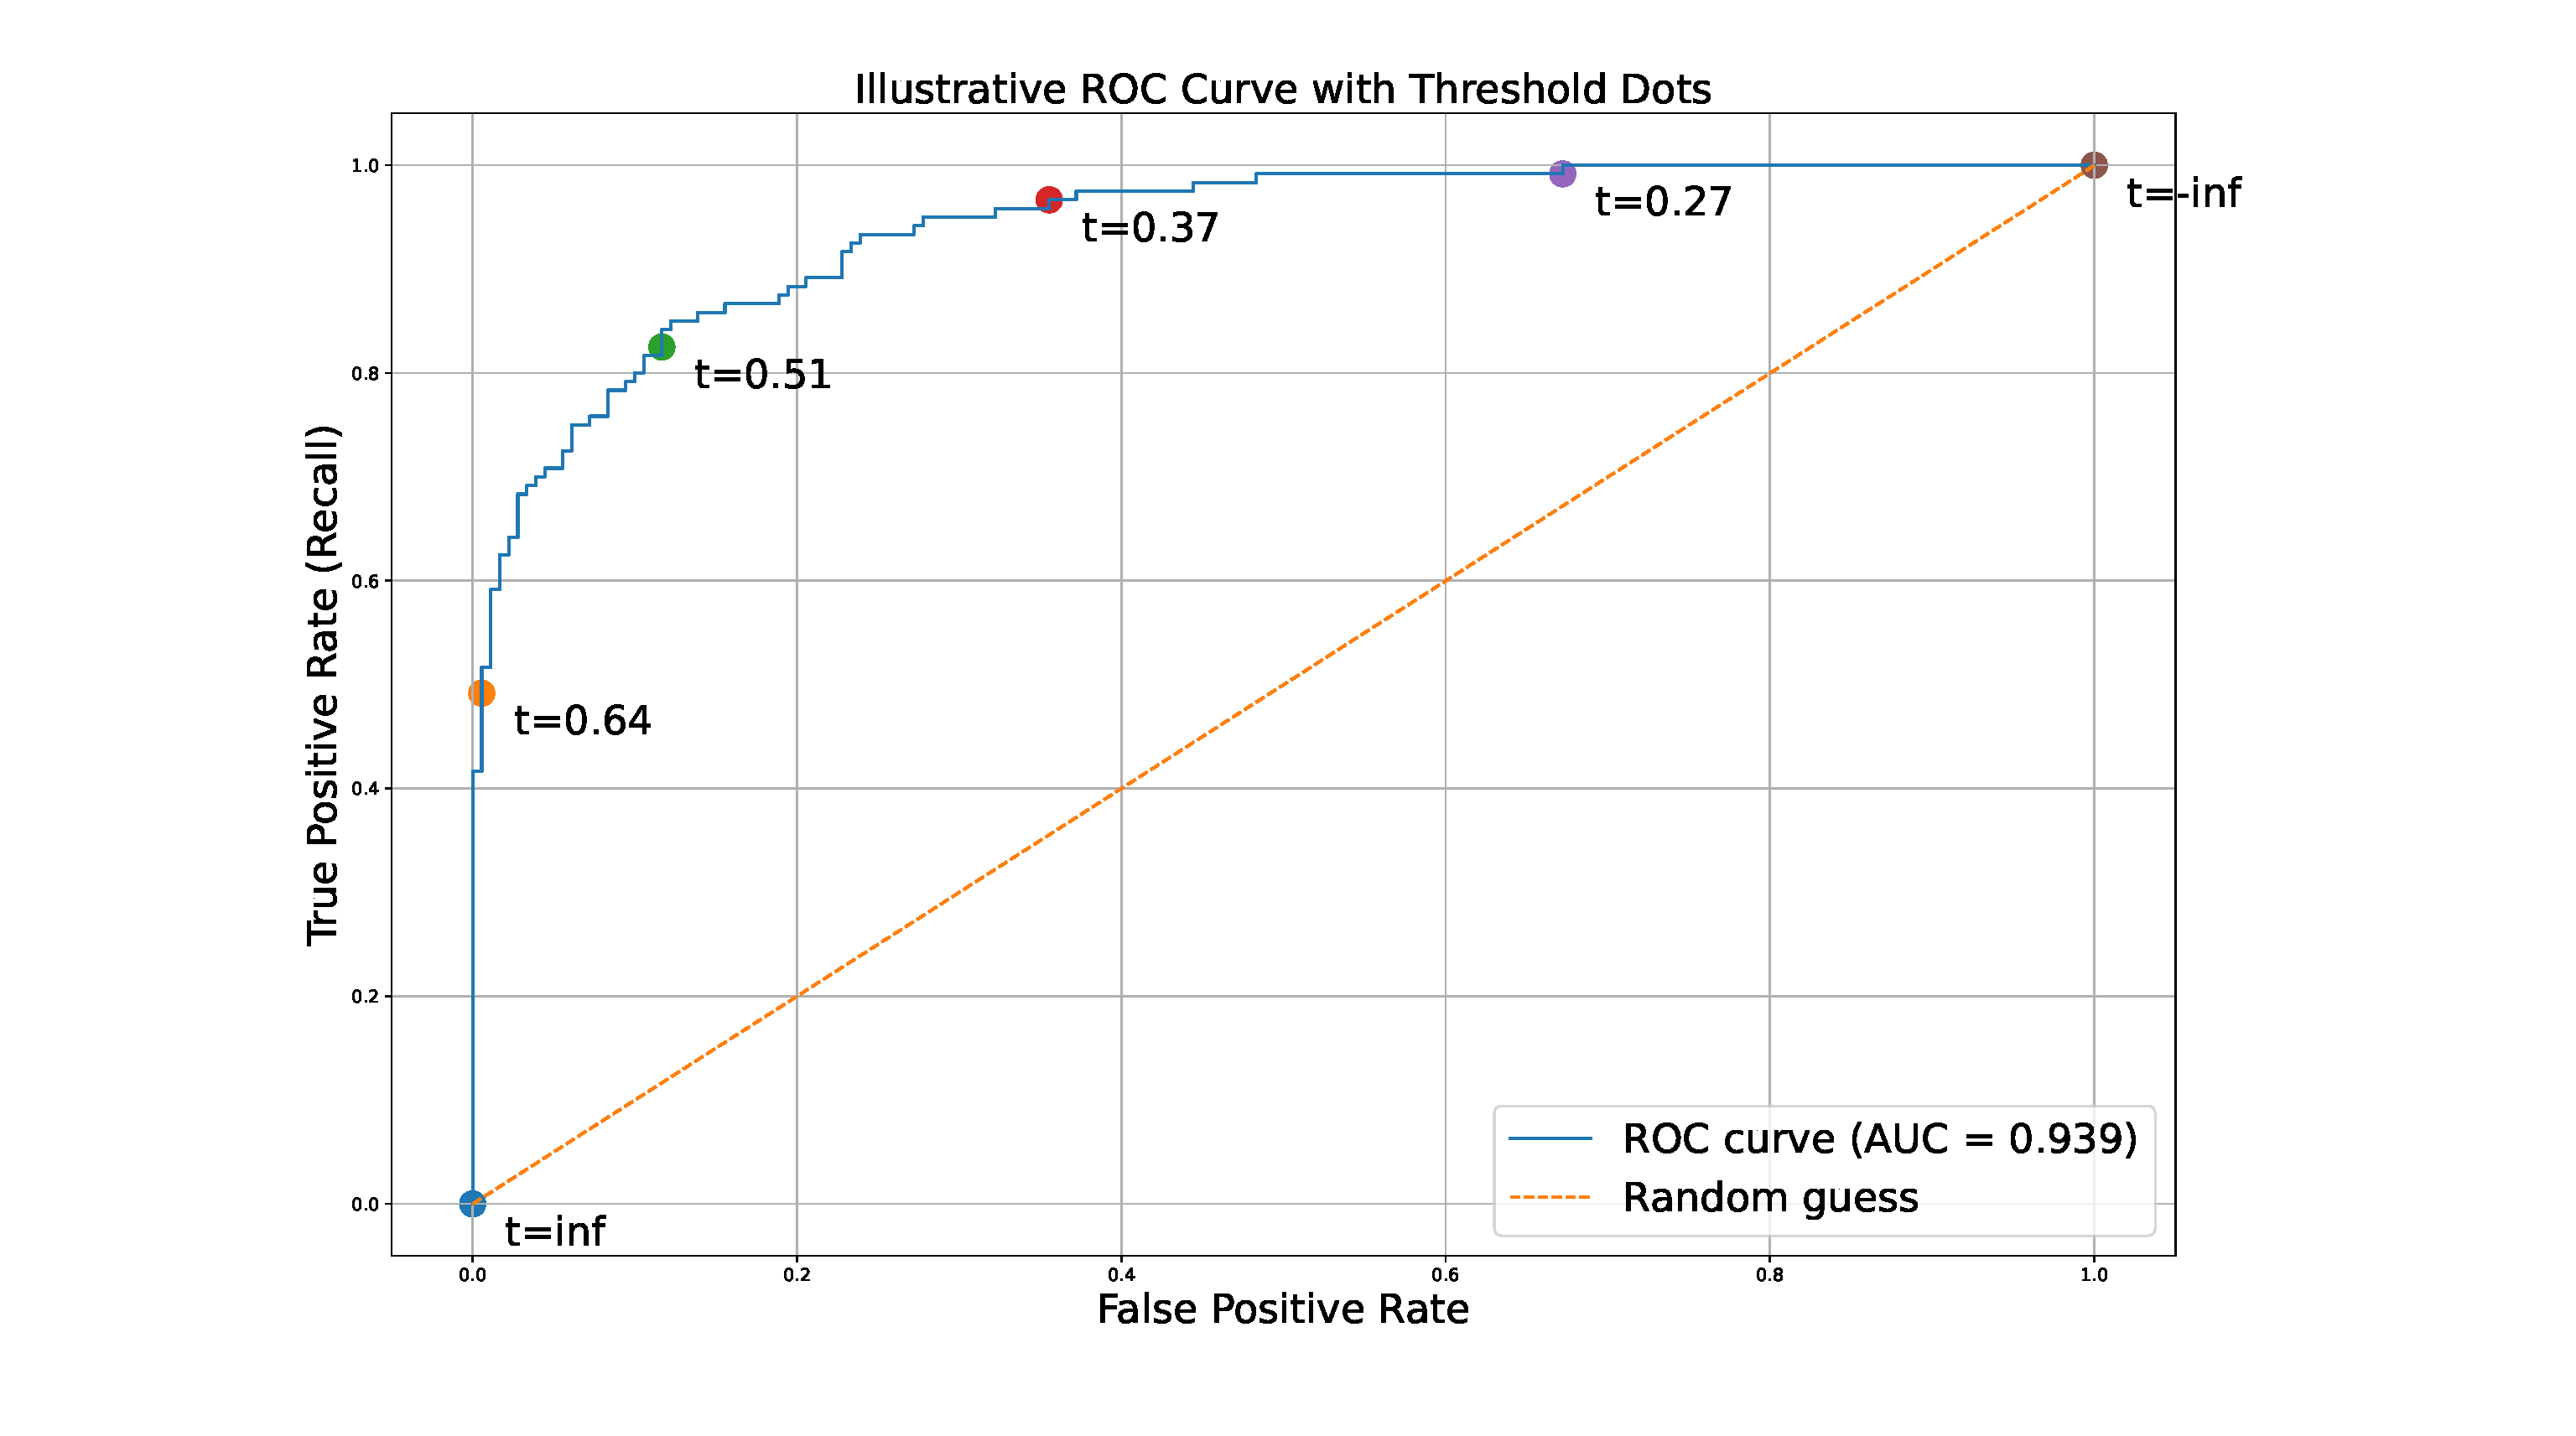
\includegraphics[scale=0.3]{./images/evaluation_metrics/roc_curve.pdf}
	\caption{Each dot on the ROC curve represents the TPR and the FPR at a specific threshold.}
\end{figure}
\begin{itemize}
	\item The diagonal line shows where the TRP = FPR.
	\item A point near $(0,1)$ is ideal: low false alarms, high detection.
	\item Higher curve = better. The \textit{AUC} (area under the ROC) summarizes performance across all thresholds (1.0 is perfect). AUC is especially helpful when we have to compare multiple models, since it provides a simple comparison. 
	\item Choose the point that best matches your costs/requirements.
\end{itemize}

\subsection{Precision Recall Graphs}

When classes are highly imbalanced, ROC curves can be misleading. With very few positives, the false positive rate (FPR) can stay low even for weak models, giving an overly optimistic picture. In these cases, precision–recall (PR) curves are more informative because they focus on the positive class: they plot precision (y-axis) versus recall (x-axis), where recall equals TPR. PR curves highlight how many of the predicted positives are actually correct (precision) at each level of coverage (recall), making them better suited for rare-event detection.

This is because precision is more informative than FPR under heavy class imbalance: precision ignores true negatives (TN), whereas FPR uses them. The illustrative plot below shows the difference.

\begin{figure}[h]
	\centering
	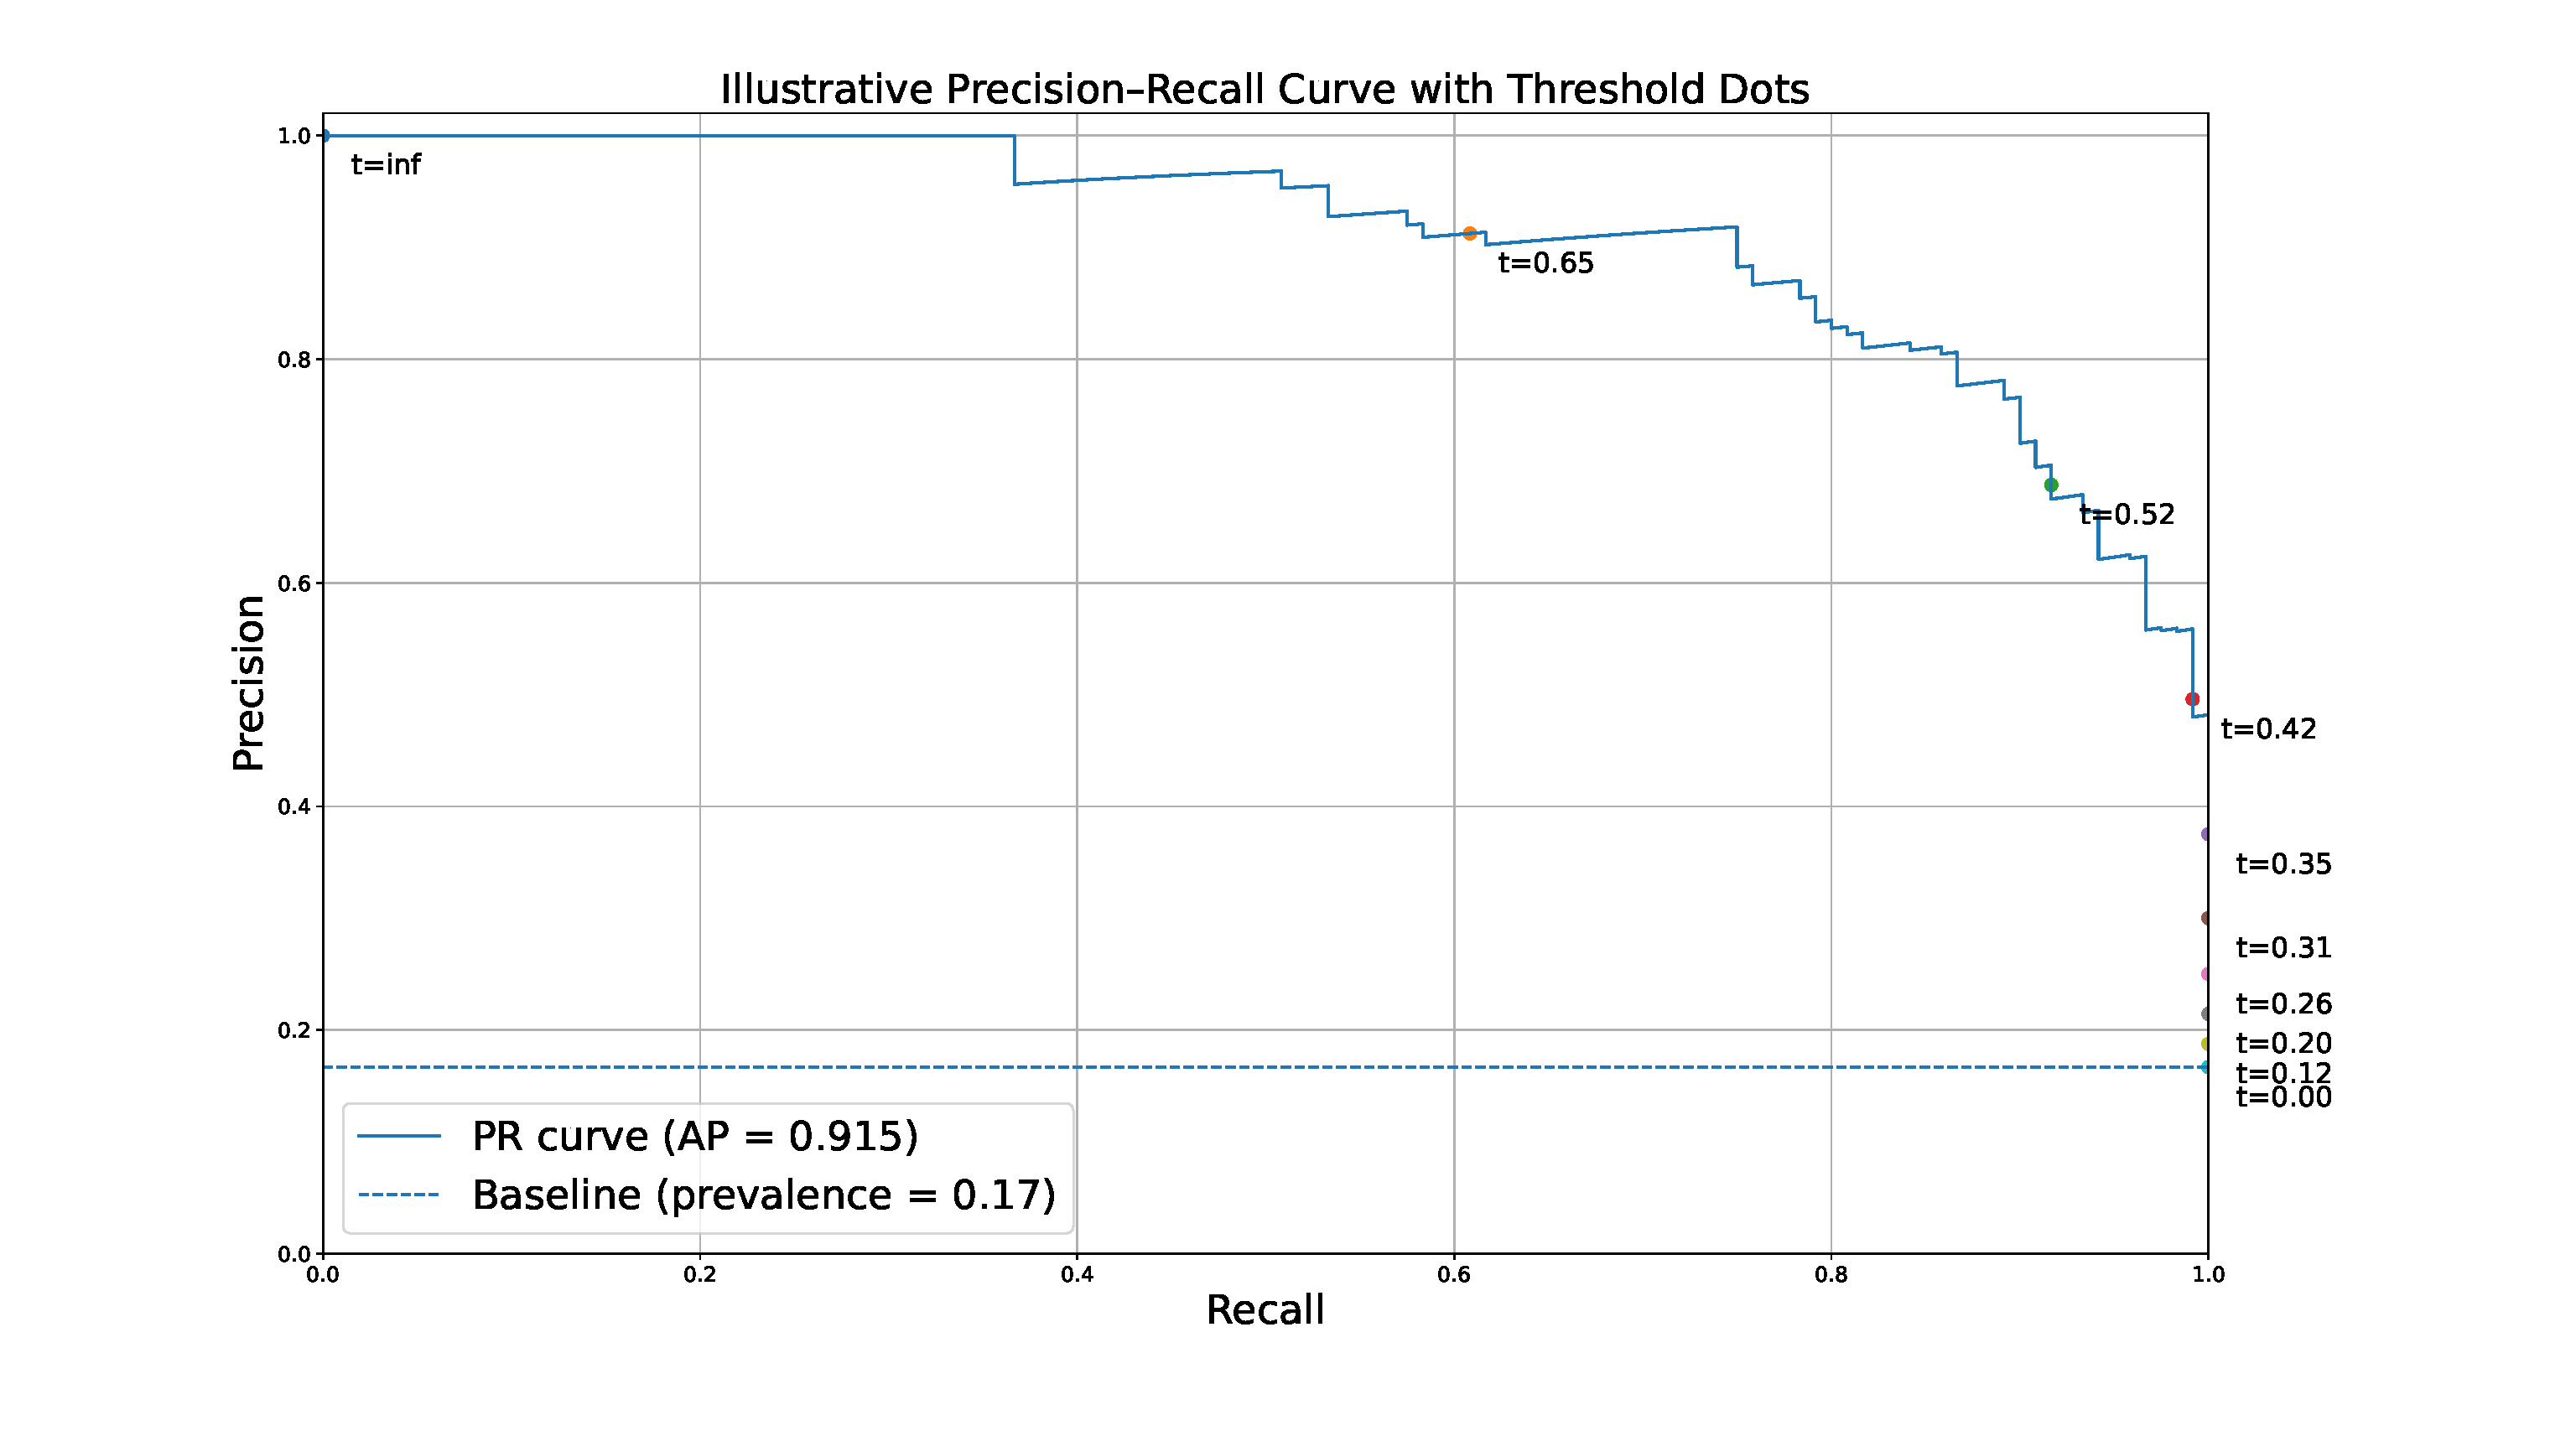
\includegraphics[scale=0.3]{./images/evaluation_metrics/pr_curve.pdf}
\end{figure}

In sum, for imbalanced data, use PR curves (precision vs recall) instead of ROC: FPR can look small simply because true negatives dominate, while PR directly measures the quality of positive predictions.

Rule of thumbs:
\begin{itemize}
	\item For rare positives or alerting workflows: use PR (and report precision@recall or recall@precision). 
	\item For balanced data or TN-sensitive views: also show ROC/AUC.
\end{itemize}

